% -*- latex -*-
%%%%%%%%%%%%%%%%%%%%%%%%%%%%%%%%%%%%%%%%%%%%%%%%%%%%%%%%%%%%%%%%
%%%%
%%%% This TeX file is part of the course
%%%% Introduction to Scientific Programming in C++/Fortran2003
%%%% copyright 2017-9 Victor Eijkhout eijkhout@tacc.utexas.edu
%%%%
%%%% array.tex : basic language elements
%%%%
%%%%%%%%%%%%%%%%%%%%%%%%%%%%%%%%%%%%%%%%%%%%%%%%%%%%%%%%%%%%%%%%

\Level 0 {Introduction}

An \indextermdef{array} is an indexed data structure, that for each
index stores an integer, floating point number, character,
object, et cetera.
In scientific applications, arrays often correspond to vectors and
matrices, potentialy of quite large size. (If you know about the
\acf{FEM}, you know that vectors can have sizes in the millions or beyond.)

In this chapter you will see the C++ \indextermtt{vector} construct,
which implements the notion of an array of things, whether they be
numbers, strings, object.

\begin{slide}{What are vectors?}
  \label{sl:what-vector}
  \begin{itemize}
  \item `Array' of items:
    \begin{itemize}
    \item items of any type (but the same for all elements of one
      vector)
    \item potentially very many items
    \end{itemize}
  \item Indexed set of items
  \item \ldots~but if you don't need the index: collection of items
  \end{itemize}
\end{slide}

While C++ can use the C~mechanisms for arrays, for almost all purposes
it is better to use \lstinline{vector}. In particular, this is a safer way to
do dynamic allocation. The old
mechanisms are briefly discussed in section~\ref{sec:staticarray}.

\begin{slide}{Vectors are better than arrays}
  \label{sl:vector-why}
  Vectors are fancy arrays. They are easier and safer to use:
  \begin{itemize}
  \item They know what their size is.
  \item Bound checking.
  \item Freed when going out of scope: no memory leaks.
  \item Dynamically resizable.
  \end{itemize}
  In C++ you never have to \indextermtt{malloc} again.\\
  (Not even \indextermtt{new}.)
\end{slide}

\Level 1 {Vector creation}

To use vectors, you first need the \lstinline{vector} header from the
\ac{STL}. Then you declare a vector, specifying what type of element
it contains. Next you may want to decide how many elements it
contains; you can specify this when you declare the vector, or
determine it later, dynamically.

\begin{block}{Vector definition}
  \label{sl:vector-def}
  Definition, mostly without initialization.
\begin{lstlisting}
#include <vector>
using std::vector;

vector<type> name;
vector<type> name(size);
vector<type> name(size,init_value);
\end{lstlisting}
where
\begin{itemize}
\item \lstinline{vector} is a keyword,
\item \n{type} (in angle brackets) is any elementary type or class
  name,
\item \n{name} is up to you, and
\item \n{size} is the (initial size of the vector). This is an integer,
  or more precisely, a \indextermtt{size_t} parameter.
\item Initialize all elements to \n{init_value}.
\end{itemize}
\end{block}

\Level 1 {Element access}

The simplest way to access vector elements is with the square bracket notation:
\begin{lstlisting}
x[1] = 3.14;
cout << x[2];
\end{lstlisting}
This gives very fast access, but there is no \emph{checking} on whether the
index is within the \emph{array
  bounds}\index{array!bounds!checking}. Accessing an element outside
the bounds may abort your code, typically with a
\indexterm{segmentation fault}, but your code may just as well
proceed, using invalid data.

As you see in this example, if \n{a}~is a vector, and \n{i} an
integer, then \n{a.at(i)} is the i'th element.
\begin{itemize}
\item The expression \n{a.at(i)} can be used to get the value of a
  vector element, or it can occur in the left-hand side of an
  assignment to set the value.
\item The \indextermbus{array}{index} (or
  \indextermbus{array}{subscript}) \n{i} starts numbering at zero.
\item Therefore, if a vector has $n$ elements, its last element has
  index~\n{n-1}.
\item If you try to get an element outside the bounds of the vector,
  the compiler will only detect this in simple cases. More likely,
  your program may give a runtime error, but that does not necessarily
  happen. You could just get some random value.
\end{itemize}

There is a safer way to access elements:
\begin{lstlisting}
x.at(1) = 3.14;
cout << x.at(2);  
\end{lstlisting}
This is slightly slower, but it does perform bounds checking for every access.

\begin{slide}{Accessing vector elements}
  \label{sl:vectorsub}
  Square bracket notation:
\begin{lstlisting}
vector<double> x(5, 0.1 );
x[1] = 3.14;
cout << x[2];
\end{lstlisting}
With bound checking:
\begin{lstlisting}
x.at(1) = 3.14;
cout << x.at(2);
\end{lstlisting}
Safer, slower.
\end{slide}

\Level 1 {Initialization}

In some applications you will create an array, and gradually fill it,
for instance in a loop. However, sometimes your elements are known in
advance and you can write them out. Specifying these values while
creating the array is called \indextermbus{array}{initialization}, and
there is more than one way to do so.

First of all, you can easily set a vector to a constant:

\begin{block}{Vector constant initialization}
  \label{sl:vector-initconst}
  There is a syntax for initializing a vector with a constant:
\begin{lstlisting}
vector<float> x(25,3.15);
\end{lstlisting}
which gives a vector of size~25, with all elements initialized to~3.15.
\end{block}

If your vector is short enough, you can set all elements explicitly with an
\indexterm{initializer list}:

\begin{block}{Vector initialization}
  \label{sl:vector-init}
  You can initialize a vector as a whole:
  %
  \snippetwithoutput{dynamicinit}{array}{dynamicinit}
\end{block}

\Level 0 {Ranging over a vector}
\label{sec:arrayrange}

If you need to consider all the elements in a vector, you typically
use a \lstinline{for} loop. There are various ways of doing this.

First of all consider the cases where you consider the vector as a
collection of elements, and the loop functions like a mathematical
`for all'.

\index{range-based for loop|see{for, range-based}}
\begin{block}{Range over elements}
  \label{sl:array-range}
  You can write a \indextermsub{range-based}{for} loop, which
  considers the elements as a collection.
\begin{lstlisting}
for ( float e : array )
  // statement about element with value e
for ( auto e : array )
  // same, with type deduced by compiler
\end{lstlisting}

\snippetwithoutput{dynamicmax}{array}{dynamicmax}
\end{block}

\begin{block}{Ranging over a vector}
  \label{sl:vector-range}
\begin{lstlisting}
for ( auto e : my_vector)
  cout << e;
\end{lstlisting}
(Technical note: \lstinline{e}~is a copy of the array element.)
\end{block}

(You can spell out the type of the vector element, but such type
specifications can be complex. In that case, using \indextermtt{auto} is
quite convenient.)

So-called \emph{initializer lists}\index{initializer list}
can also be used as a list denotation:

\begin{block}{Range over vector denotation}
  \label{sl:range-denote}
  \snippetwithoutput{rangedenote}{array}{rangedenote}  
\end{block}

If you actually need the index of the element, you can use a
traditional \lstinline{for} loop with loop variable.

\begin{block}{Indexing the elements}
  \label{sl:index-range}
  You can write an \indextermsub{indexed}{for} loop, which uses an
  index variable that ranges from the first to the last element.
\begin{lstlisting}
for (int i= /* from first to last index */ )
  // statement about index i
\end{lstlisting}
Example: find the maximum element in the array, and where it occurs.
%
\snippetwithoutput{vecidxmax}{array}{vecidxmax}
\end{block}

\begin{exercise}
  \label{ex:range-for}
  Indicate for each of the following vector operations whether you
  prefer to use an indexed loop or a range-based loop. Give a short
  motivation.
  \begin{itemize}
  \item Count how many elements of a vector are zero.
  \item Find the location of the last zero.
  \end{itemize}
\end{exercise}

\begin{exercise}
  \label{ex:array-max}
  Find the element with maximum absolute value in a vector. Use:
\begin{lstlisting}
vector<int> numbers = {1,-4,2,-6,5};
\end{lstlisting}
% Which mechanism do you use for traversing the vector?

Hint:
\begin{lstlisting}
#include <cmath>
..
absx = abs(x);
\end{lstlisting}
\end{exercise}

\begin{exercise}
  \label{ex:array-maxidx}
  Find the location of the first negative element in a vector.

  Which mechanism do you use?
\end{exercise}

\begin{exercise}
  \label{ex:array-sorted}
  Check whether a vector is sorted.
\end{exercise}

\begin{block}{Range over elements by reference}
  \label{sl:array-range-ref}
  Range-based loop indexing makes a copy of the vector element. If you
  want to alter the vector, use a reference:
  %
\begin{lstlisting}
for ( auto &e : my_vector)
  e = ....
\end{lstlisting}
%
\snippetwithoutput{vectorrangeref}{array}{vectorrangeref}

(Can also use \lstinline{const auto& e} to prevent copying, but also
prevent altering data.)
\end{block}

\begin{exercise}
  If you do the prime numbers project, you can now do exercise~\ref{sec:arraysieve}.
\end{exercise}

\begin{block}{Indexing with pre/post increment}
  \label{sl:prepostindex}
Indexing in \lstinline{while} loop and such:
\begin{lstlisting}
x = a.at(i++); /* is */ x = a.at(i); i++;
y = b.at(++i); /* is */ i++; y = b.at(i);
\end{lstlisting}
\end{block}

\begin{block}{Example of increment indexing}
  \snippetwithoutput{plusplustest1}{loop}{plusplus}
  %
  Exercise: modify this so that after the while loop \n{index} is the
  number of leading odd elements.
\end{block}

\Level 0 {Vector are a class}
\label{sec:stdvector}

You wouldn't tell it from the above examples, but vectors actually
form a \indextermttdef{vector} class. You can have a vector of ints,
floats, doubles, et cetera; 
the angle bracket notation indicates what the specific type stored in
the vector is.
You could say that the vector class is parametrized with the type (see
chapter~\ref{ch:template} for the details). We could say that
\lstinline{vector<int>} is a new data type, pronounced `vector-of-int', and you can
make variables of that type.

\begin{block}{Vector copy}
  \label{sl:vectorcopy}
  Vectors can be copied just like other datatypes:
  %
  \snippetwithoutput{vectorcopy}{array}{vectorcopy}
\end{block}

\Level 1 {Vector methods}

There are several \emph{methods}\index{vector!methods}
to the \lstinline{vector} class. Some of the simpler ones are:
\begin{itemize}
\item \lstinline{at}: index an element
\item \lstinline{size}: give the size of the vector
\item \lstinline{front}: first element
\item \lstinline{back}: last element
\end{itemize}

There are also methods relating to dynamic storage management, which
we will get to next.

\begin{exercise}
  \label{ex:vectornormalize}
  Create a \n{vector} $x$ of \lstinline{float} elements, and set them to random
  values.

  Now normalize the vector in $L_2$ norm and check the correctness of
  your calculation, that is,
  \begin{enumerate}
  \item Compute the $L_2$ norm of the vector:
    \[ \| v\| \equiv \sqrt{\sum_iv_i^2} \]
  \item Divide each element by that norm;
  \item The norm of the scaled vector should now by~1. Check this.
  \end{enumerate}
  What type of loop are you using?
\end{exercise}

\begin{slide}{Vector methods}
  \label{sl:vector-method}
  \begin{itemize}
  \item Get elements, including bound checking, with
    \lstinline{ar.at(3)}.
    Note: (zero-based indexing).
  \item (also get elements with \lstinline{ar[3]}: see later discussion.)
    %% (for C programmers: this is not dereferencing, this uses an
    %% operator method)
  \item Size: \lstinline{ar.size()}.
  \item Other functions: \lstinline{front}, \lstinline{back}, \lstinline{empty}.
  \item \lstinline{vector} is a `templated class':
    \lstinline{vector<X>} is a vector-of-\lstinline{X}.
  \end{itemize}
\end{slide}

\Level 1 {Vectors are dynamic}
\label{sec:stdvector-dynamic}

A vector
can be grown or shrunk after its creation.
For instance, you can use the \lstinline{push_back} method to add elements at the end:

\begin{block}{Dynamic vector extension}
  \label{sl:vector-dynamic}
  Extend with \indextermtt{push_back}:
  %
  \snippetwithoutput{vectorpush}{array}{vectorend}
  %
  also \lstinline{pop_back}, \lstinline{insert}, \lstinline{erase}.\\
  Flexibility comes with a price.
\end{block}

It is tempting to use \lstinline{push_back} to create a vector dynamically.

\begin{block}{Dynamic size extending}
  \label{sl:vector-extend}
\begin{lstlisting}
vector<int> iarray;
\end{lstlisting}
creates a vector of size zero. You can then
\begin{lstlisting}
iarray.push_back(5);
iarray.push_back(32);
iarray.push_back(4);
\end{lstlisting}
\end{block}

However, this dynamic resizing involves memory management, and maybe
operating system functions. This will probably be
inefficient. Therefore you should use such dynamic mechanisms only
when strictly necessary.
If you know the size,
create a vector with that size. If the size is not precisely known but
you have a reasonable upper bound, you can 
reserve the vector at that size:
\begin{lstlisting}
vector<int> iarray;
iarray.reserve(100);
while ( ... )
  iarray.push_back( ... );
\end{lstlisting}

\Level 0 {Vectors and functions}

\Level 1 {Pass vector to function}

\begin{block}{Vector as function argument}
  \label{sl:vector-arg}
  You can pass a vector to a function:
\begin{lstlisting}
void print0( vector<double> v ) {
  cout << v.at(0) << endl;
};
\end{lstlisting}
Vectors, like any argument, are passed by value, so the vector is
actually copied into the function.
\end{block}

\begin{block}{Vector pass by value example}
  \label{sl:vector-arg-ex}
  \snippetwithoutput{vectorpassval}{array}{vectorpassnot}  
\end{block}

\begin{exercise}
  \label{ex:vectornormalize-function}
  Revisit exercise~\ref{ex:vectornormalize} and introduce a function
  for computing the $L_2$ norm.
\end{exercise}

\begin{block}{Vector pass by reference}
  \label{sl:vector-arg-ref}
  If you want to alter the vector, you have to pass by reference:
  %
  \snippetwithoutput{vectorpassref}{array}{vectorpassref}  
\end{block}

\begin{exercise}
  \label{ex:vec-rand-sort}
  Write functions \n{random_vector} and \n{sort} to make the following
  main program work:
\begin{lstlisting}
int length = 10;
vector<float> values = random_vector(length);
vector<float> sorted = sort(values);
\end{lstlisting}
  This creates a vector of random values of a specified length, and
  then makes a sorted copy of it.

  The alternative would in-place sorting. Find
  arguments for/against that approach.

\end{exercise}

(See section~\ref{sec:crand} for the random fuction.)

Passing a vector by reference means that the subprogram becomes able
to alter it. To prevent that, pass it as a
\indextermsub{const}{reference}; section~\ref{sec:const-ref}.

\Level 1 {Vector as function return}

\begin{block}{Vector as function return}
  \label{sl:vector-return}
  You can have a vector as return type of a function.\\
  Example: this function
  creates a vector, with the first element set to the size:
  %
  \snippetwithoutput{vectorreturn}{array}{vectorreturn}
\end{block}

\begin{exercise}
  \label{ex:vec-of-squares}
  Write a function of one \lstinline{int} argument~$n$, which returns vector
  of length~$n$, and which contains the first $n$ squares.
\end{exercise}

\begin{exercise}
  \label{ex:splitoddeven}
  Write code to take a vector of integers, and construct two
  vectors, one containing all the odd inputs, and one containing all
  the even inputs. So:
\begin{lstlisting}
input:
   5,6,2,4,5
output:
   5,5
   6,2,4
\end{lstlisting}
  Can you write a function that accepts a vector and produces two
  vectors as described?
\end{exercise}

\Level 0 {Vectors in classes}

You may want an object that contains a vector, where the size of the
vector is passed to the constructor. Since the class definition is an
abstract definition of all possible objects, clearly you can not have the
vector size there.

\begin{lstlisting}
class witharray {
private:
  vector<int> the_array( ???? );
public:
  witharray( int n ) {
    thearray( ???? n ???? );
  }
}
\end{lstlisting}

\begin{slide}{Can you make a class around a vector?}
  \label{sl:class-with-vector}
  Vector needs to be created with the object, so you can not have the
  size in the class definition
\begin{lstlisting}
class witharray {
private:
  vector<int> the_array( ???? );
public:
  witharray( int n ) {
    thearray( ???? n ???? );
  }
}
\end{lstlisting}
\end{slide}

The solution is to specify a vector without size in the class
definition, which creates a vector of size zero. When you create an
object, you then create a vector of the right size, and use that as
the vector member of the object.

\begin{block}{Create and assign}
  \label{sl:class-has-vector}
  The following mechanism works:
\begin{lstlisting}
class witharray {
private:
  vector<int> the_array;
public:
  witharray( int n )
    : the_array(vector<int>(n)) {
  };
};
\end{lstlisting}
Better than
\begin{lstlisting}
  witharray( int n ) {
    the_array = vector<int>(n);
  };
\end{lstlisting}
\end{block}

The two cases behave slightly differently.
\begin{itemize}
\item The expression \lstinline{vector<int>(n)} creates an anonymous vector
  of size~\lstinline{n};
  \begin{itemize}
  \item In the first case, that anonymous vector is moved to become
    the value of the \n{the_array} variable;
  \item in the second case, the object is first created with
    \n{the_array} being an empty
    vector, and the size-$n$ is then written over it. This is less
    efficient and less elegant.
  \end{itemize}
\item Either way, now you have an object with a vector of size~\n{n} internally.
\end{itemize}

\Level 1 {Timing}

Different ways of acessing a vector can have drastically different
timing cost.

\begin{block}{Filling in vector elements}
  \label{sl:vect-extend-code}
  You can push elements into a vector:
  \verbatimsnippet{vectorflex}

  If you allocate the vector statically, you can assign with \n{at}:
  \verbatimsnippet{vectorat}
\end{block}

\begin{block}{Filling in vector elements}
  \label{sl:vect-extend-code2}
  With subscript:
  \verbatimsnippet{vectorsub}

  You can also use \indextermtt{new} to allocate:
  %
  \verbatimsnippet{vectornew}
  %
  (note: legacy C mechanism. Do not use)
\end{block}

For \indextermtt{new}, see section~\ref{sec:cnew}. However, note that
this mode of allocation is basically never needed.

Timings are partly predictable, partly surprising:
\begin{block}{Timing the ways of filling a vector}
  \label{sl:vector-extend-time}
\begin{lstlisting}
  Flexible time: 2.445
  Static at time: 1.177
  Static assign time: 0.334
  Static assign time to new: 0.467
\end{lstlisting}
\end{block}

The increased time for \lstinline{new} is a mystery.

So do you use \lstinline{at} for safety or \lstinline{[]} for speed? Well, you could
use \lstinline{at} during development of the code, and insert
\begin{lstlisting}
#define at(x) operator[](x)
\end{lstlisting}
for production.

\Level 0 {Wrapping a vector in an object}

You may want to a create objects that contain a vector, for instance
because you want to add some methods.
%
\verbatimsnippet{printablevector}

Unfortunately this means you may have to recreate some methods:
%
\verbatimsnippet{vectorinheritat}

\Level 0 {Multi-dimensional cases}

Unlike Fortran, C++ has little support for multi-dimensional
arrays. If your multi-dimensional arrays are to model linear algebra
objects, it would be good to check out the \indexterm{Eigen}
library. Here are some general remarks on multi-dimensional storage.

\Level 1 {Matrix as vector of vectors}

\begin{block}{Multi-dimensional vectors}
  \label{sl:multi-vector}
  Multi-dimensional is harder with vectors:
\begin{lstlisting}
vector<float> row(20);
vector<vector<float>> rows(10,row);
// alternative:
vector<vector<float>> rows(10);
for ( auto &row : rows )
  row = vector<float>(20);
\end{lstlisting}
Create a row vector, then store 10 copies of that:\\
vector of vectors.
\end{block}

This is not the best implementation of a matrix, for instance because
the elements are not contiguous. However, let's continue with it for a moment.

\begin{block}{Matrix class}
  \label{sl:matrix-class}
  \verbatimsnippet{matrixclassdef}
\end{block}

\begin{exercise}
  \label{ex:matrixclass-rowcol1}
  Write \n{rows()} and \n{cols()} methods for this class that return
  the number of rows ad columns respectively.
\end{exercise}

\begin{exercise}
  \label{ex:matrix-methods}
  Add methods such as \n{transpose}, \n{scale} to your matrix class.

  Implement matrix-matrix multiplication.
\end{exercise}

\Level 1 {A better matrix class}

You can make a `pretend' matrix by storing a long enough \n{vector} in
an object:
%
\verbatimsnippet{matrixclass}

\begin{slide}{Matrix class'}
  \label{sl:matrix-class-cont}
  Better idea:
\begin{lstlisting}
  elements = vector<double>(rows*cols);
  ...
  void get(int i,int j) {
    return elements.at(i*cols+j);
  }
\end{lstlisting}
(Old-style solution: use cpp macro)
\end{slide}

\begin{exercise}
  \label{ex:matrixclass-rowcol2}
  Why are \lstinline{m,n} here stored explicitly, and not in the
  previous case?
\end{exercise}

The most important advantage of this is that it is compatible with
the storage traditionally used in 
many libraries and codes.

The syntax for \n{set} and \n{get} can be improved.
\begin{exercise}
  Write a method \n{element} of type \n{double&}, so that you can write
\begin{lstlisting}
A.element(2,3) = 7.24;
\end{lstlisting}
\end{exercise}

\Level 0 {Advanced topics}

\Level 1 {Iterators}
\label{sec:iterator}

You have seen how you can iterate over a vector
\begin{itemize}
\item by an indexed loop over the indices, and
\item with a range-based loop over the indices.
\end{itemize}
There is a third way, which is actually the basic mechanism underlying
the range-based looping.

An \indexterm{iterator} is, in a metaphorical sense (see
section~\ref{sec:iterator-class} for details) a pointer to a vector
element. Mirroring the index-loop convention of
\begin{lstlisting}
for (int i=0; i<hi; i++)
  element = vec.at(i);
\end{lstlisting}
you can iterate:
\begin{lstlisting}
for (auto elt_ptr=vec.begin(); elt_ptr!=vec.end(); ++elt_ptr)
  element = *elt_ptr;
\end{lstlisting}
Some remarks:
\begin{itemize}
\item This is one of the very few places where you need the asterisk in C++
  for \indexterm{dereferencing}; section~\ref{sec:cderef}. (However,
  the thing you are dereferencing is an iterator, not a pointer.)
\item As with a normal loop, the \n{end} iterator point just beyond the end
  of the vector.
\item You can do \indextermbus{pointer}{arithmetic} on iterators, as
  you can see in the \verb-++elt_ptr- update part of the loop header.
\end{itemize}
Another illustration of pointer arithmetic on iterators is getting the
last element of a vector:
%
\snippetwithoutput{vectorpush}{array}{vectorend}
\snippetwithoutput[vectorend]{vectorpushiterator}{array}{vectorenditerator}

\Level 1 {Old-style arrays}
\label{sec:staticarray}

Static arrays are really an abuse of the equivalence of arrays and
addresses of the C programming language. This appears for instance in
parameter passing mechanisms.

For small arrays you can use a different syntax. 

\snippetwithoutput{arrayinit}{array}{staticinit}

This has the
(minimal) advantage of not having the overhead of a class
mechanism. On the other hand, it has a number of disadvantages:
\begin{itemize}
\item You can not query the size of an array by its name: you have to
  store that information separately in a variable.
\item Passing such an array to a function is really passing the
  address of its first element, so it is always (sort of) by
  reference.
\end{itemize}

Range-based indexing works the same as with vectors:
%
\snippetwithoutput{rangemax}{array}{rangemax}

\Level 2 {C-style arrays and subprograms}

Arrays can be passed to a subprogram, but the bound is unknown there.
%
\verbatimsnippet{arraypass}
%
\begin{exercise}
  Rewrite the above exercises where the sorting tester or the maximum
  finder is in a subprogram.
\end{exercise}

Unlike with scalar arguments, array arguments can be altered by a
subprogram: it is as if the array is always passed by reference. This is
not strictly true: what happens is that the address of the first
element of the array is passed. Thus we are really dealing with pass
by value, but it is the array address that is passed rather than its value.

\Level 2 {Multi-dimensional arrays}

Multi-dimensional arrays can be declared and used with a simple extension of
the prior syntax:
\begin{lstlisting}
float matrix[15][25];

for (int i=0; i<15; i++)
  for (int j=0; j<25; j++)
    // something with matrix[i][j]
\end{lstlisting}

Passing a multi-dimensional array to a function, only the first
dimension can be left unspecified:
%
\verbatimsnippet{arraypass2d}

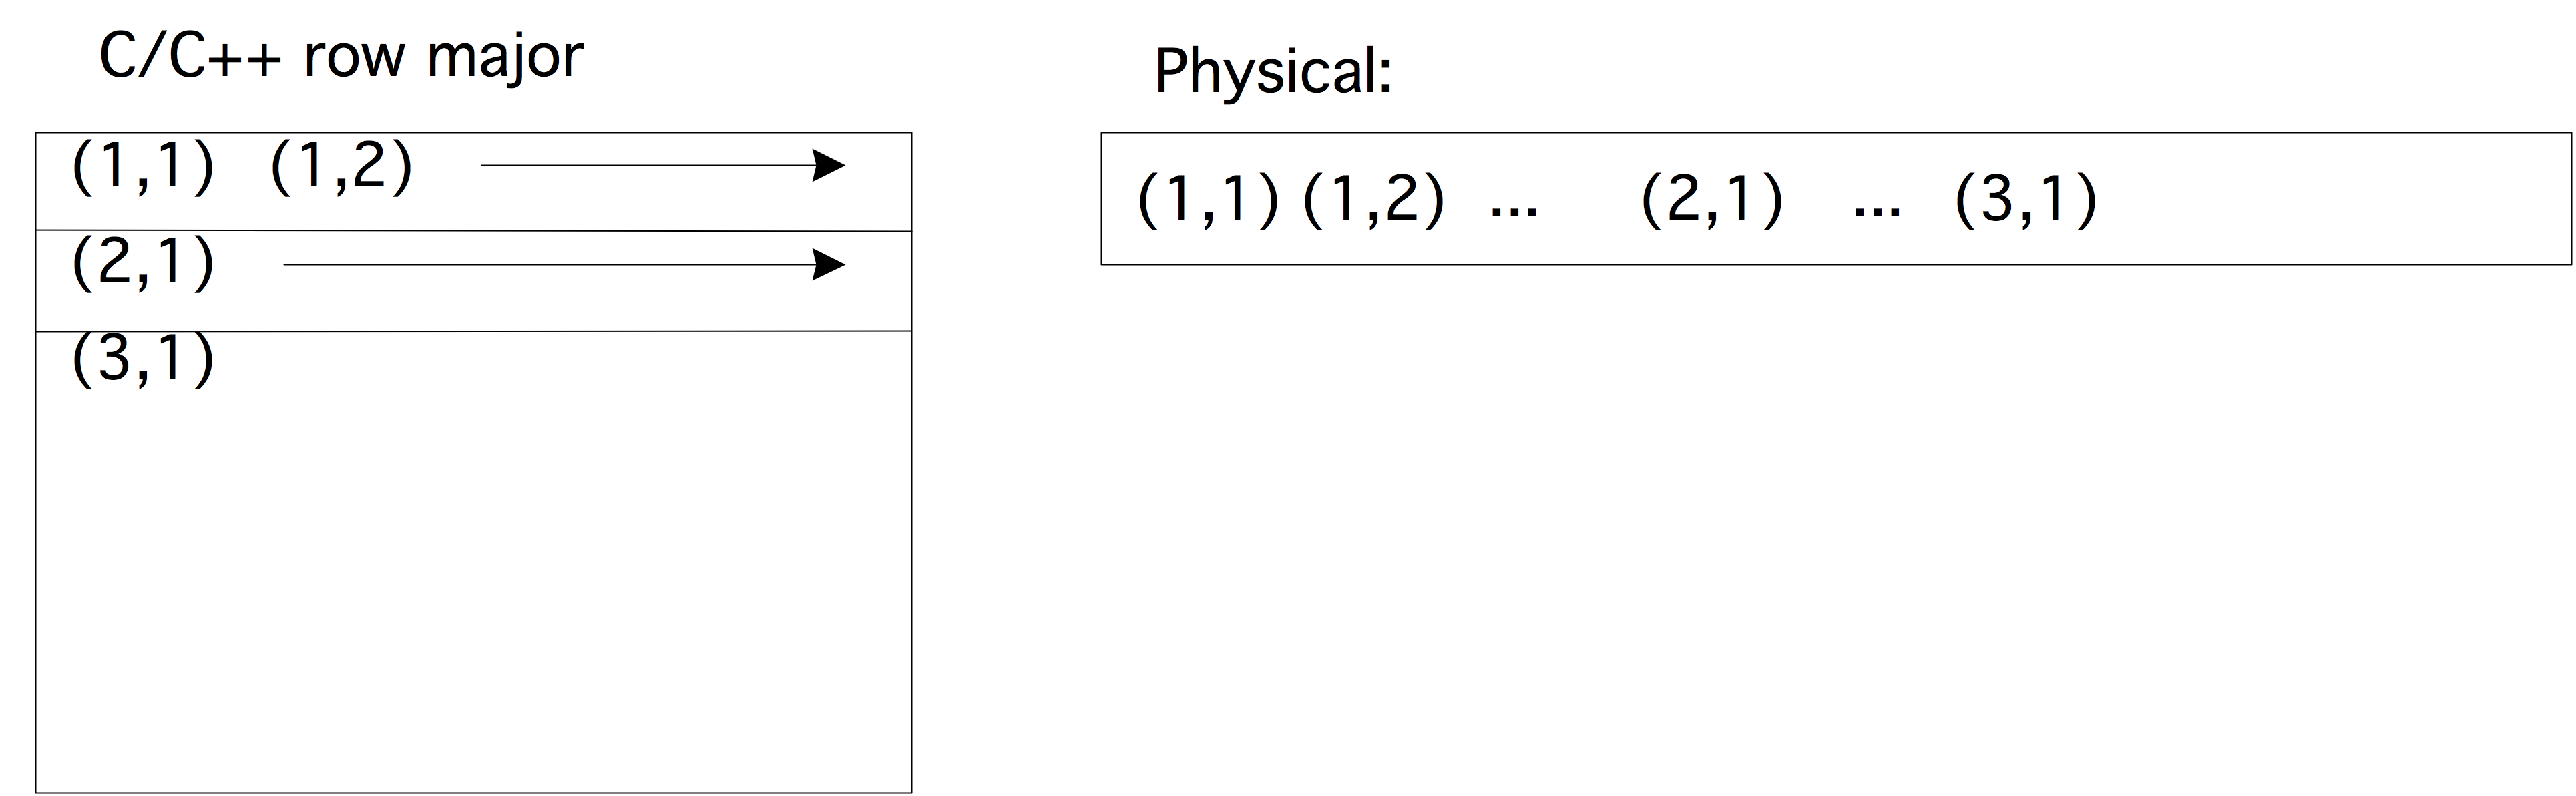
\includegraphics[scale=.1]{arrayc}

\Level 2 {Memory layout}

Puzzling aspects of arrays, such as which dimensions need to be
specified and which not in a function call, can be understood by
considering how arrays are stored in memory.
The question then is how a two-dimensional (or higher dimensional)
array is mapped to memory, which is linear.
\begin{itemize}
\item A one-dimensional array is stored in contiguous memory.
\item A two-dimensional array is also stored contiguously, with first
  the first row, then the second, et cetera.
\item Higher dimensional arrays continue this notion, with contiguous
  blocks of the highest so many dimensions.
\end{itemize}

As a result of this, indexing beyond the end of a row, brings you to the
start of the next row:
%
\verbatimsnippet{arraywrap}

We can now also understand how arrays are passed to functions:
\begin{itemize}
\item The only information passed to a function is the address of the
  first element of the array;
\item In order to be able to find location of the second row (and
  third, et cetera), the subprogram needs to know the length of each
  row.
\item In the higher dimensional case, the subprogram needs to know the
  size of all dimensions except for the first one.
\end{itemize}

\Level 1 {Stack and heap allocation}
\label{sec:stack-heap}

The concepts of \indexterm{stack} and \indexterm{heap} do not appear
in the \indextermbus{C++}{standard}. However, the following
description generally applies:
\begin{itemize}
\item Objects that obey scope are allocated on the stack, so that
  their memory is automatically freed control leaves the scope.
\item Dynamically created objects, such as the target of a pointer,
  live on the heap because their lifetime is not subject to scope.
\end{itemize}
The existence of the second category is a source of
\indextermbus{memory}{leak}s in languages such as~C. This danger is
greatly lessened in~C++.

While in C the only way to create dynamic objects is by a call to
\indextermtt{malloc}, in C++ a \indextermtt{vector} obeys scope, and
therefore lives on the stack. If you wonder if this may lead to
\indextermbus{stack}{overflow}, rest assured: only the descriptor, the
part of the vector that remembers the size, is on the stack, while the
actual data is on the heap. However, it is no longer subject to memory
leaking, since the heap storage is deallocated when the vector object
goes out of scope.

If you want heap memory that transcends scope you can use the
\indextermsub{smart}{pointer} mechanism, which also guarantees against
memory leaks. See chapter~\ref{pointer}.

\Level 1 {The Array class}

In cases where an array will never change size it would be convenient
to have a variant of the \lstinline{vector} class that does not have
the dynamic memory management facility.
The \indextermttdef{array} class seems to fulfill this role at first sight.
However, it
is limited to arrays where the size is known at compile time.

\Level 1 {Span}
\label{sec:gsl-span}

The old C~style arrays allowed for some operations that are harder to
do with vectors. For instance, you could create a subset of an array with:
\begin{lstlisting}
double *x = (double*)malloc(N*sizeof(double));
double *subx = x+1;
subx[1] = 5.; // same as: x[2] = 5.;
\end{lstlisting}
In C++ you can write
\begin{lstlisting}
vector<double> x(N);
vector<double> subx( x.begin()+1,x.end() );
\end{lstlisting}
but that allocates new storage.

If you really want two vector-like objects to share data there is the
\indextermttdef{span} class, which is in the \ac{STL} of
\emph{C++20}\index{C++!C++20}. Until this standard is available you
can use the \indexac{GSL}, for instance implemented in
\url{https://github.com/Microsoft/GSL}.

A span is little more than a pointer and a size, so it allows for the
above use case. Also, it does not have the overhead of creating a
whole new vector.

\begin{block}{Span}
  \label{sl:spandef}
\begin{lstlisting}
vector<double> v;
auto v_span = gsl::span<double>( v.data(),v.size() );
\end{lstlisting}
The \indextermtt{span} object has the same \lstinline{at}, \lstinline{data}, and
\lstinline{size} methods, and you can iterate over it, but it has no
dynamic methods.
\end{block}

\Level 0 {Exercises}

\begin{exercise}
  Given a vector of integers, write two loops;
  \begin{enumerate}
  \item One that sums all even elements, and
  \item one that sums all elements with even indices.
  \end{enumerate}
  Use the right type of loop.
\end{exercise}

\begin{exercise}
  Program \indexterm{bubble sort}: go through the array comparing
  successive pairs of elements, and swapping them if the second is
  smaller than the first. After you have gone through the array, the
  largest element is in the last location. Go through the array again,
  swapping elements, which puts the second largest element in the
  one-before-last location. Et cetera.
\end{exercise}

\begin{block}{Pascal's triangle}
  \label{sl:pascal-def}
  \small
  \indexterm{Pascal's triangle} contains binomial coefficients:
{\scriptsize
\begin{verbatim}
Row    1:                     1
Row    2:                   1   1
Row    3:                 1   2   1
Row    4:               1   3   3   1
Row    5:             1   4   6   4   1
Row    6:           1   5  10  10   5   1
Row    7:         1   6  15  20  15   6   1
Row    8:       1   7  21  35  35  21   7   1
Row    9:     1   8  28  56  70  56  28   8   1
Row   10:   1   9  36  84 126 126  84  36   9   1
\end{verbatim}
}
where \[ p_{rc} = \begin{pmatrix} r\\c \end{pmatrix} = \frac{r!}{c!(r-c)! }. \]
The coefficients can easily be computed from the recurrence
\[ p_{rc} = 
\begin{cases}
  1&c\equiv 1\vee c\equiv r\\
  p_{r-1,c-1}+p_{r-1,c}
\end{cases}
\]
\end{block}

\begin{exercise}
  \label{ex:pascal-ex}
  \small
  \begin{itemize}
  \item 
    Write a class \n{pascal} so that \n{pascal(n)} is the object
    containing $n$~rows of the above coefficients. Write a method
    \n{get(i,j)} that returns the $(i,j)$ coefficient.
  \item
    Write a method \n{print} that prints the above display.
  \item
    Write a method \n{print(int m)} that prints a star if the
    coefficient modulo~$m$ is nonzero, and a space otherwise.
\begin{verbatim}
          *
         * *
        *   *
       * * * *
      *       *
     * *     * *
    *   *   *   *
   * * * * * * * *
  *               *
 * *             * *
\end{verbatim}
  \item
    The object needs to have an array internally. The easiest solution
    is to make an array of size $n\times n$.
  \end{itemize}
\end{exercise}

\begin{exercise}
  \label{ex:pascal-ey}
  Extend the Pascal exercise:\\
  Optimize your code to use
  precisely enough space for the coefficients.
\end{exercise}

\begin{exercise}
  A knight on the chess board moves by going two steps horizontally or
  vertically, and one step either way in the orthogonal
  direction. Given a starting position, find a sequence of moves that
  brings a knight back to its starting position. Are there starting
  positions for which such a cycle doesn't exist?
\end{exercise}

\begin{exercise}
  Put eight queens on a chessboard so that none threatens any other.
\end{exercise}

\begin{exercise}
  From the `Keeping it REAL' book, exercise 3.6 about Markov chains.
\end{exercise}
